%% ****** Start of file template.aps ****** %
%%
%%
%%   This file is part of the APS files in the REVTeX 4 distribution.
%%   Version 4.0 of REVTeX, August 2001
%%
%%
%%   Copyright (c) 2001 The American Physical Society.
%%
%%   See the REVTeX 4 README file for restrictions and more information.
%%
%
% This is a template for producing manuscripts for use with REVTEX 4.0
% Copy this file to another name and then work on that file.
% That way, you always have this original template file to use.
%
% Group addresses by affiliation; use superscriptaddress for long
% author lists, or if there are many overlapping affiliations.
% For Phys. Rev. appearance, change preprint to twocolumn.
% Choose pra, prb, prc, prd, pre, prl, prstab, or rmp for journal
%  Add 'draft' option to mark overfull boxes with black boxes
%  Add 'showpacs' option to make PACS codes appear
\documentclass[aps,prl,twocolumn,showpacs,superscriptaddress,groupedaddress]{revtex4}  % for review and submission
%\documentclass[aps,preprint,showpacs,superscriptaddress,groupedaddress]{revtex4}  % for double-spaced preprint
\usepackage{graphicx}  % needed for figures
\usepackage{dcolumn}   % needed for some tables
\usepackage{bm}        % for math
\usepackage{amssymb}   % for math
 \usepackage{comment} % for large comment sections
\usepackage{color}
\usepackage[percent]{overpic}

\usepackage{amsmath}


% avoids incorrect hyphenation, added Nov/08 by SSR
\hyphenation{ALPGEN}
\hyphenation{EVTGEN}
\hyphenation{PYTHIA}


\begin{document}

% The following information is for internal review, please remove them for submission
\widetext
\leftline{Version 0 as of \today}
\leftline{Primary authors: Elena Gramellini}
\leftline{To be submitted to PRD.}
\leftline{Comment to {\tt elenag@fnal.gov} by xxx, yyy}
\centerline{\em LArIAT INTERNAL DOCUMENT -- NOT FOR PUBLIC DISTRIBUTION}

% the following line is for submission, including submission to the arXiv!!
%\hspace{5.2in} \mbox{Fermilab-Pub-04/xxx-E}

\title{Measurement of the ($\pi^-$, Ar) total hadronic cross section at the LArIAT experiment}
\input lariat_author_list.tex       % LArIAT authors (remove the first 3 lines
                                       % of this file prior to submission, they
                                       % contain a time stamp for the authorlist)
                                       % (includes institutions and visitors)
\date{\today}


\begin{abstract}
We present the first measurement of the negative pion total hadronic cross section on argon in the 100-1050 MeV kinetic energy range as performed at the Liquid Argon In A Testbeam (LArIAT)  experiment. LArIAT deploys a Liquid Argon Time Projection (LArTPC) on a beam of charged particles at the Fermilab Test Beam Facility (FTBF). 
For this measurement, we select and measure the pions from the beam and we develop the ``thin slice method" --  a new technique to measure cross sections at LArTPCs.  Our measurement of the  ($\pi^-$,Ar) total hadronic cross section is in agreement with the predictions by the Geant4  model in the 350-1050 MeV region, while a shape difference arises at lower energies.
The ($\pi^-$, Ar) total cross-section has never been measured before; the outcome of this measurement will enable to quantify and reduce the systematic associated with the hadronic interaction models in neutrino-argon interactions in current and future LAr experiments such as the Short Baseline Neutrino Program and DUNE.\\

 \end{abstract}

\pacs{13.15.+g Neutrino interactions, 14.40.-n	Mesons,  14.40.Be	Light mesons (S=C=B=0), 13.75.-n	Hadron-induced low- and intermediate-energy reactions and scattering (energy $le$ 10 GeV)}
\maketitle

\newpage
\section{\label{sec:Motivations}Motivations}
In this work, we measured  for the first time the total hadronic cross section of negative pions on argon in the energy region between 100 and 1050 MeV. We briefly review here the findings on pion hadronic cross sections from historic measurements on lighter and heavier nuclei performed in the seventies.  Now, a renewed interest for hadronic cross sections -- particularly cross sections on argon -- arises in light of the modern neutrino experiments landscape. Compared to the historic measurements, LArIAT developed a new  methodology to measure cross sections on argon which has the potential to meet this renewed interest. 

\subsection{Historic Measurements of Pion Hadronic Cross Sections: Lighter and Heavier Nuclei}
Many experiments with pion beams have studied the hadronic interaction of pions on light and heavy nuclei, such as  He, Li, C, Fe, Pb \cite{Wilkin:1973xd, Clough1974,PhysRevC.14.635}, albeit never on argon.  Most historic measurements of pion hadronic cross sections are performed on thin targets. At their core, these experiments consists in shooting a beam of pions with a known flux on a thin slab of material and recording the outgoing flux; flux conservation allows to retrieve the interacting flux and to calculate the cross section at the beam energy.
In this work, we developed a complementary approach called ``the thin slice method". Contrary to thin target experiments, we shoot pions on a thick but fully sensitive target  -- the LArTPC -- and we directly record the interacting flux. 

Regardless of the nuclear medium, the shape of the pion-nucleus interaction cross section in the energy range accessible to our measurement shows the distinct features indicating the presence of a resonance. In fact, the mean free path of a pion of kinetic energy between 100 and 400 MeV is much shorter than the average distance between nucleons (which is of the order of a
 1 fm),   enhancing the pion interaction probability with surface nucleons. A delta resonance is often produced in the interaction, which subsequently decays inside the nucleus.
Historical experimental results show a dependency of the delta resonance shape as a function of the nuclear mass number \cite{PhysRevC.14.635}. The delta resonance shape becomes less pronounced  
and its peak shifts to lower energies when the nuclear mass number increases; this effect is due to kinematic considerations and to the difference in propagation of the delta inside the nucleus. Multiple scattering effects modify the resonance width, which is larger than the natural-decay width.


\subsection{\label{sec:Sign} $\pi^{-}$Ar Hadronic Interactions: Signal Signatures}
Strong hadronic interaction models \cite{9780198520085,9780471779957} predict the pion interaction processes with argon in the hundreds of MeVs energy range. 
The total hadronic ($\pi^{-}$,Ar) interaction cross section defines the probability of a single hadronic process on argon.  In measuring the total cross section, we include both the elastic interactions with interaction angle greater than 5 deg and  the reaction channel, 
\begin{equation}
\sigma_{Tot} = \sigma_{Elastic}+ \sigma_{Reaction}; 
\end{equation}
the limit on the interaction angle is driven by the resolution of the LArIAT tracking.
The reaction channel can be further characterized by several exclusive channels with defined topologies,
\begin{equation}
\sigma_{Reaction} = \sigma_{Inelastic} + \sigma_{abs} + \sigma_{chex}+ \sigma_{\pi prod};
\end{equation}
in this work, we account for all reaction channels, regardless of their final state. Upcoming measurements from LArIAT will focus on the reaction exclusive channels.
Figure \ref{fig:PionsEvd} shows examples of topologies for pion-argon hadronic interactions as they appear in the  LArIAT data: elastic and inelastic scattering, pion absorption with emission of protons, charge exchange and production of pions.


\begin{figure}
  \centering  
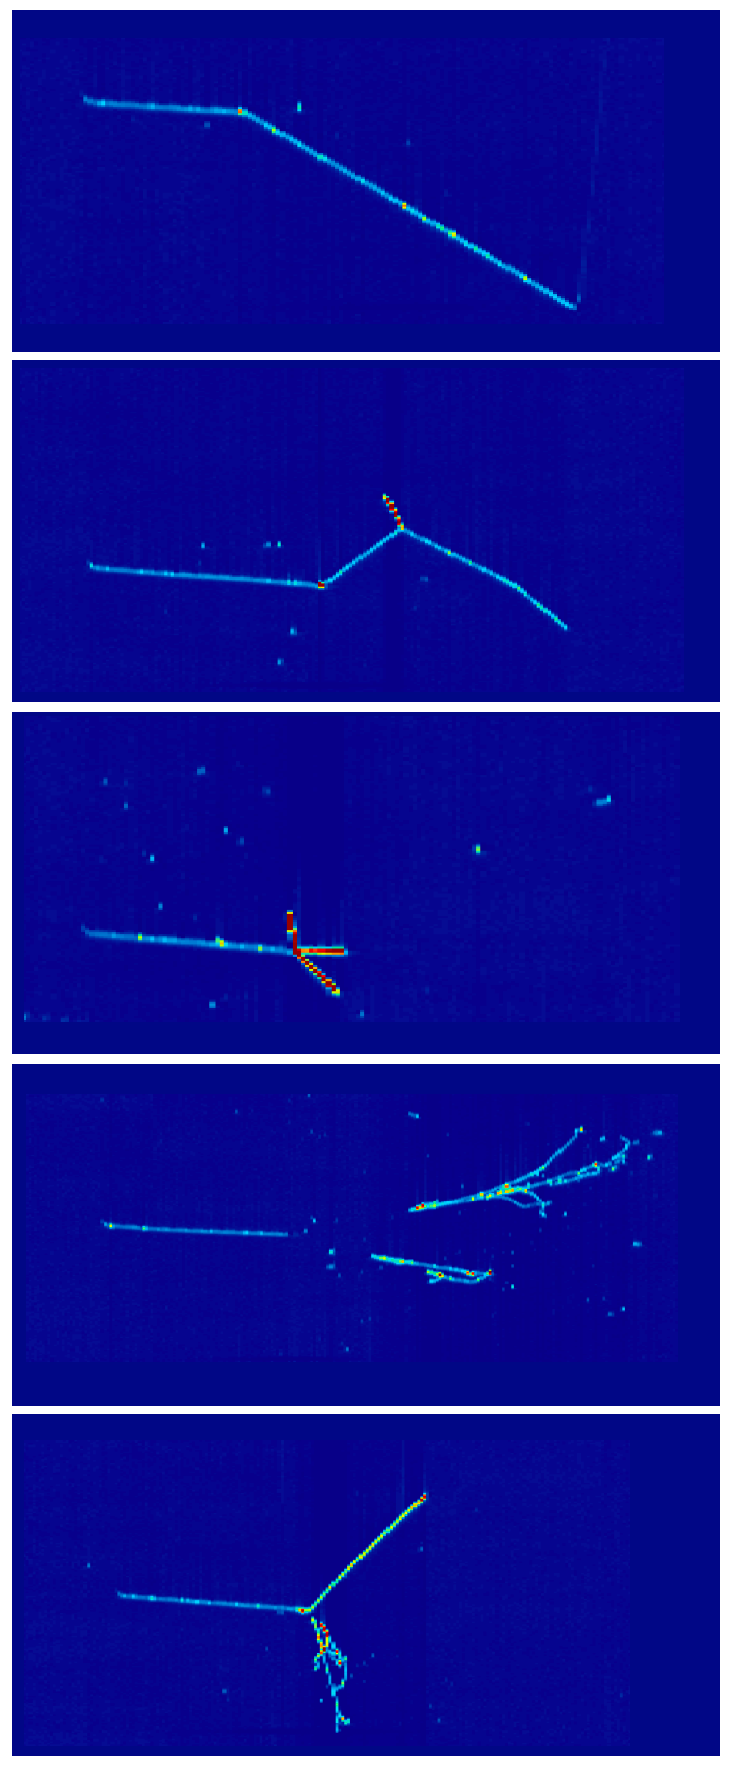
\includegraphics[width =0.5\textwidth]{Evds}
\caption{Pion-Argon interaction topologies due to elastic scattering, inelastic scattering, pion absorption with emission of protons, charge exchange and production of pions as seen in the LArIAT data. The event displays show the raw signals in the wire vs time space for the collection plane only.}
\label{fig:PionsEvd}
\end{figure}




\subsection{$\pi^{-}$Ar Cross Section in the Context of Neutrino Searches}
Experiments based on neutrino detection relay on the products of the neutrino interaction to identify the interaction type and to reconstruct  the neutrino flavor and energy.  Pions are a common product of neutrino interactions, especially in interactions such as resonant scattering, DIS and coherent pion production.  In today's neutrino physics landscape, argon detectors are a very popular technology choice due to their ability to record extremely detailed events with high statistics. Yet, the literature on particles' interaction on argon for energies relevant to the neutrino products, namely below  1 GeV, is scarce. There are two main reasons why understanding pion hadronic interactions is important for neutrino experiments: to model the behavior of the pion inside the complex nuclear matter  and to model the behavior of the pion during its propagation inside the detector medium.  Neutrino event generators and detector simulation packages base their pion transportation for argon on the interpolations of the historical cross section measurements for lighter and heavier nuclei: the goal of LArIAT's dedicated measurement is to bridge this gap in data, thus reducing the uncertainties related to pion interactions on argon.
Assumptions on the nuclear modeling and on the interaction of hadrons inside the nucleus performed at the level of the neutrino event generator bridge the measurement of the products of a neutrino interaction to the reconstruction of the neutrino energy and flavor. In particular, hadron cross sections on argon are used in the modeling of final state interaction to determine if the hadron escapes the nuclear medium.
Once the pion has left the target nucleus, the pion-argon hadronic cross section also plays an important role in the pion transportation inside the argon medium: processes such as pion absorption or pion charge exchange can greatly modify the topology of a neutrino interaction	 in the detector and lead to significant modifications in the event classification.
Being able to reconstruct the details of pions inside the detector is an imperative for modern argon neutrino experiments to achieve the design resolution for their key physics measurements.





\section{\label{sec:ExperimentalSetup}Measurement Setup}
The LArIAT experiment consists in a LArTPC deployed on a beam of charged particles at the Fermilab Test Beam Facility (FTBF) on the  Meson Center beam line. The experimental setup changed significantly during LArIAT's three seasons of data taking in both its beamline and LArTPC components. We acquired the data used in this work  during the 24-weeks of data taking of the second season, which we refer as to Run II.  

We briefly describe here only the features and use of the LArIAT Run II  detectors  relevant to the cross section measurement; we also describe here the TPC event reconstruction, simulation packages and beamline event selection used in this analysis.  We refer the reader to \cite{LArIATDet} for a detailed description of LArIAT's experimental setup.

\subsection{\label{sec:Beamline}Beamline} 
\begin{figure*}
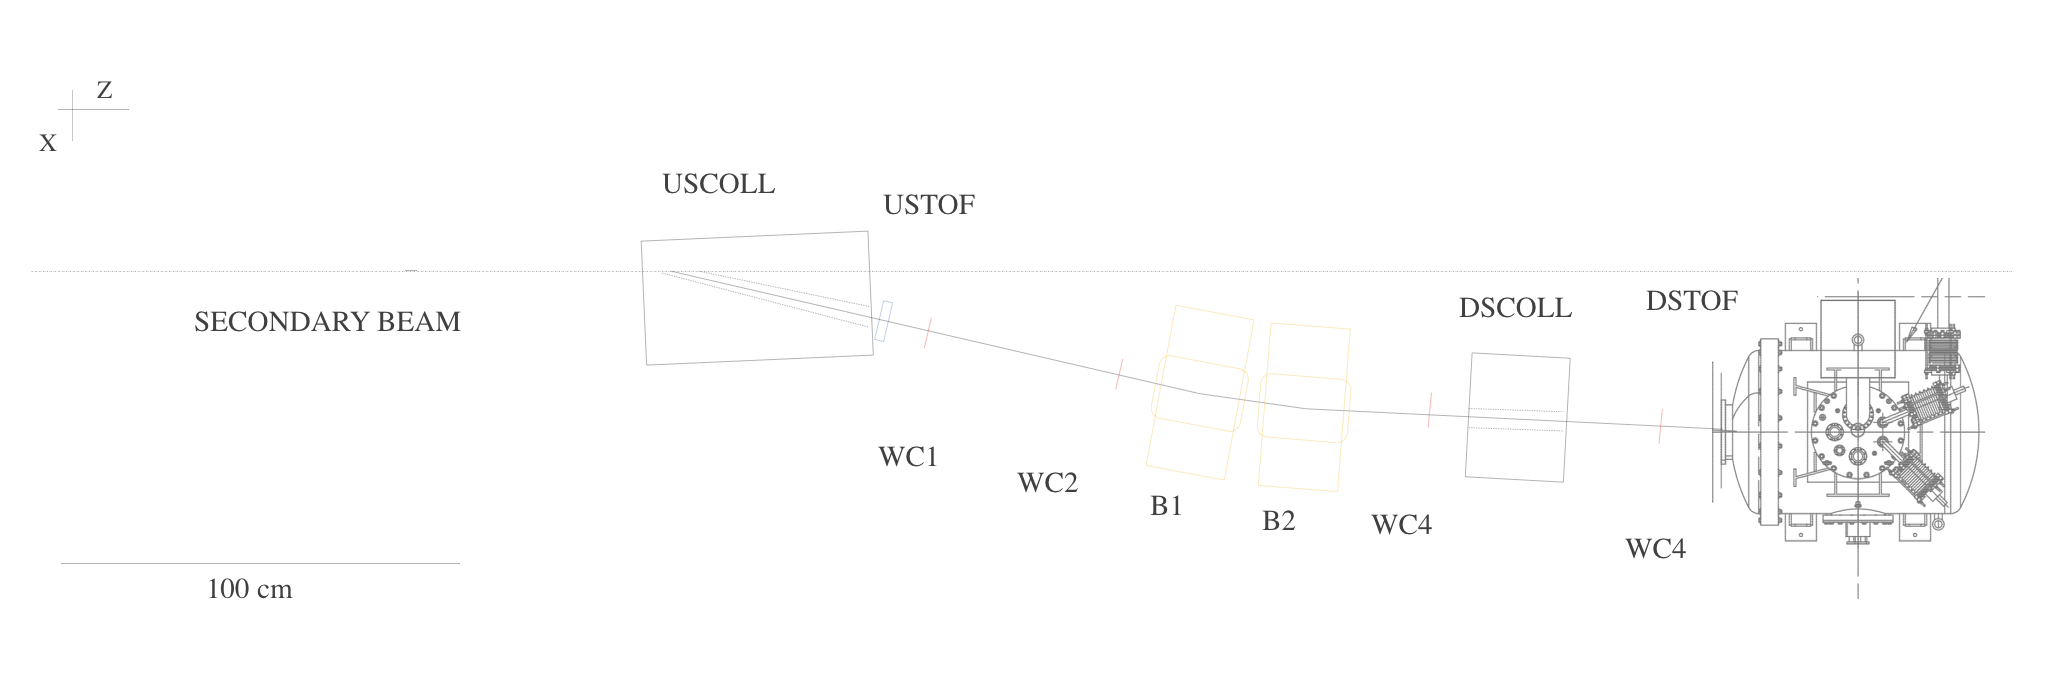
\includegraphics[width=\textwidth,height=\textheight,keepaspectratio]{Tertiary.png}
\caption{Bird's eye view of the LArIAT tertiary beamline. USCOLL and DSCOLL represent the upstream and downstream collimators respectively; B1 and B2 represent the bending magnets; WC1, WC2, WC3 and WC4 are the multi wire proportional chambers; USTOF and DSTOF represent the upstream and downstream time of flight; TPC shows the technical drawing of the cryostat which surrounds the liquid argon time projection chamber.}
\label{fig:beamlinebird}
\end{figure*}


%\begin{overpic}[width=0.5\textwidth,grid,tics=10]{momentumPiMuE.png}
% \put (20,85) {\huge$\displaystyle\gamma$}
%\end{overpic}

%The strength for the magnetic field is set by the amplitude of the current in the magnets. For this work,  the current settings employed were -60A %(B $\sim$0.21 T) 
%and -100A. %(B $\sim$0.35 T)  

LArIAT takes advantage of the Fermilab accelerator infrastructure to create its beam of charged particles.  The Fermilab accelerator complex  delivers a  primary beam of 120~GeV protons with variable intensity to the Meson Center beam line in supercycles of 60 seconds. This primary beam is focused onto a tungsten target to create a secondary beam. The secondary beamline is tuned such that the composition of the secondary particle beam is mainly positive pions. For the data considered in this work, the tunable momentum peak of the secondary beam was fixed at 64~GeV/c; this configuration assures a stable beam delivery at the LArIAT experimental hall (MC7).

At MC7, the secondary beam impinges  on a copper target within a steel collimator to create the LArIAT tertiary beam. Scope of the LArIAT tertiary beamline instrumentation is to identify the particle type and measure the momentum of the beam's particles entering the LArTPC. Figure \ref{fig:beamlinebird} shows a bird's eye view of the LArIAT tertiary beamline:  two bending electromagnets (yellow), a set of four wire chambers (red) and two time-of-flight scintillating paddles (blue).  The magnets' polarity determines the charge of the particles selected in the tertiary beam: running the magnets in negative polarity selects negatively charged particles. The tunable magnetic field strength determines the range of momentum of the beamline particles steered towards the TPC. For this work, we selected a low energy and high energy tune. 
The combination of magnets and wire chambers forms the LArIAT spectrometer which measures the particles' momentum at the fourth wire chamber, $p_{\text{Beam}}$, with a relative uncertainty of 2\%. Figure \ref{fig:momentum} shows the distribution of  $p_{\text{Beam}}$ for the Run II negative polarity data used in this work, low energy tune on the left, high energy tune on the right. The momentum range of the two datasets combined spans from $\sim200$ to $\sim1200$ MeV/c. 
%\begin{comment}     
\begin{figure}
  \centering  
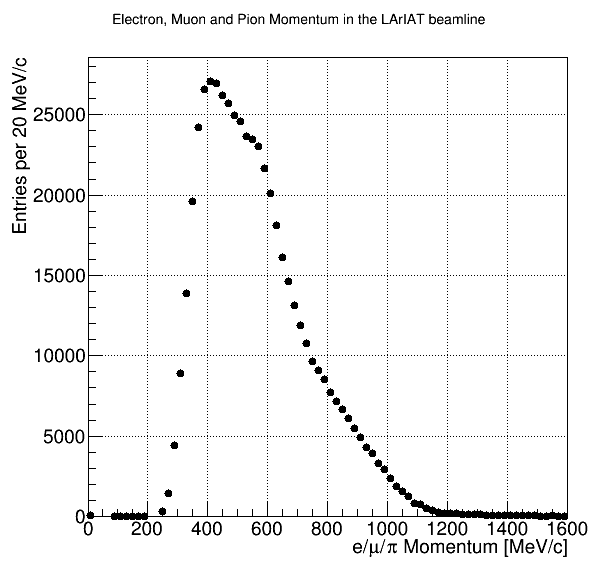
\includegraphics[width =0.4\textwidth]{momentumPiMuE.png}
\caption{Momentum spectrum in the LArIAT beamline  for Run II negative polarity data, low energy tune on the right, high energy tune on the left. \textcolor{red}{(change this figure to 2 for the low and high energy, prettyfy)}}
\label{fig:momentum}
\end{figure}



We leverage the measurement of the momentum in conjunction with the measurement of the time of flight (TOF) to calculate the particle's invariant mass $m_{\text{Beam}}$ as 
\begin{equation}
m_{\text{Beam}} = \frac{p_{\text{Beam}}}{c}\sqrt{\biggl(\frac{\text{TOF}*c}{l}\biggr)^2 -1},
\label{eq:mass}
\end{equation}
 where $c$ is the speed of light and $l$ is the length of the particle's trajectory between the time of flight paddles. 





Figure \ref{fig:mass} shows the distribution of the invariant mass for the Run II negative polarity runs. We classify beamline events into the different categories as follows:

\begin{tabular}{lllrl}
& & & &\\
 $\pi/\mu/e$: &                               & $m_{\text{Beam}}<$& 350~MeV/c$^2$&\\
 kaon:           & 350~MeV/c$^2 <$ & $m_{\text{Beam}}<$& 650~MeV/c$^2$&\\
 antiproton:   & 650~MeV/c$^2 <$ & $m_{\text{Beam}}<$& 3000~MeV/c$^2$&.\\
& & & &\\
\end{tabular}


%\begin{itemize}
%\item[-] $\pi/\mu/e$:  $m_{\text{Beam}}<$ 350~MeV/c$^2$
%\item[-] kaon: 350~MeV $< m_{\text{Beam}} <$ 650~MeV/c$^2$
%\item[-] antiproton: 650~MeV $<m_{\text{Beam}}<$ 3000~MeV/c$^2$.
%\end{itemize}

It should be noted that pions are the main component of the LArIAT beam of negatively charged particle and that the sole use of the aforementioned beamline instrumentation does not allow to discriminated between electrons, muons and pions. We make use of the topological difference between tracks and electromagnetic showers in the LArTPC  to mitigate the presence of electrons in the pion sample. A small contamination of electrons and muons still remains, which we account for as beamline background in the cross section measurement.

%\begin{comment}     
\begin{figure}
  \centering  
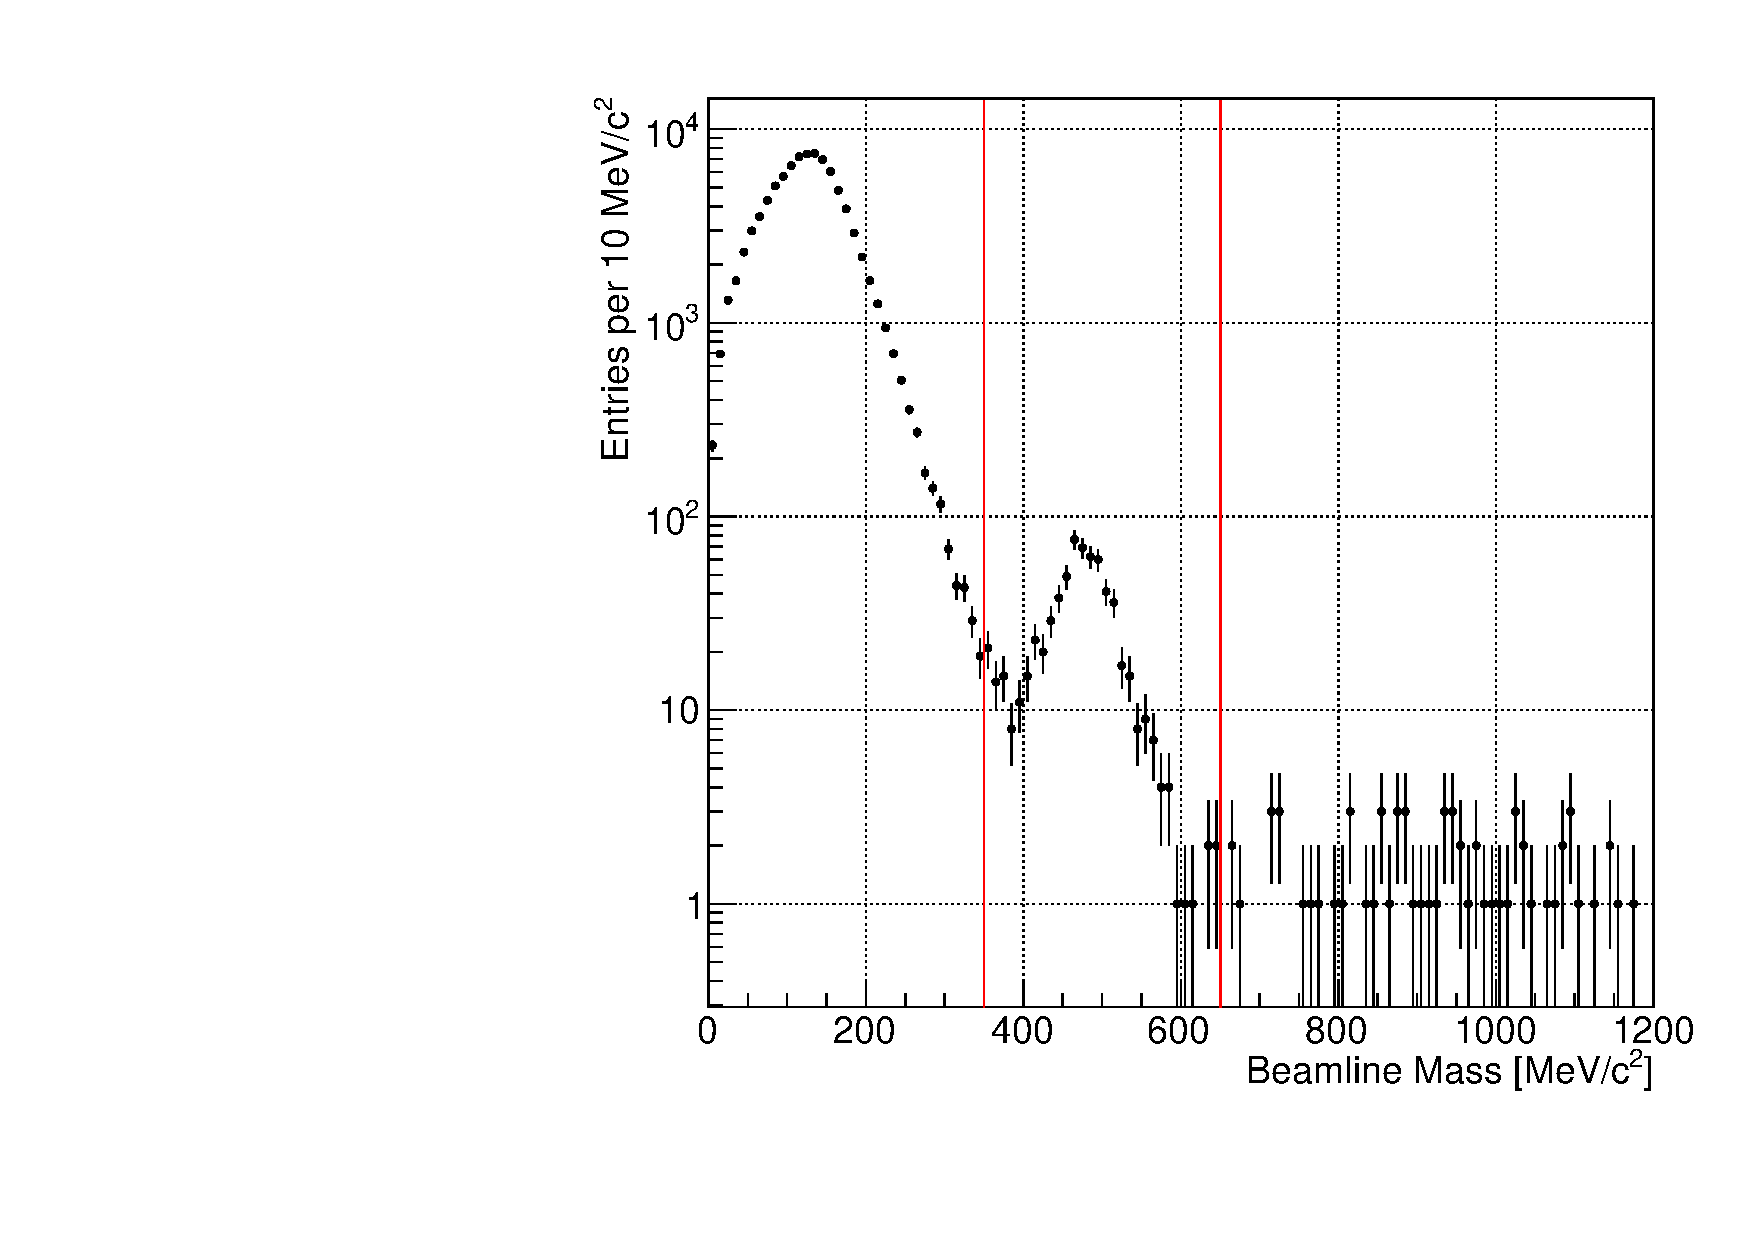
\includegraphics[width =0.4\textwidth]{massRunII.pdf}
\caption{Distribution of the beamline mass as calculated according to Equation \ref{eq:mass} for the Run-II events reconstructed in the beamline, negative polarity runs. The classification of the events into $\pi^-/ \mu^-/e^-$, K$^-$, or antiproton is based on these distributions, whose selection values are represented by the vertical colored lines.}
\label{fig:mass}
\end{figure}


\subsection{\label{sec:LArTPC}LArTPC}

The LArIAT LArTPC is a box of dimensions 47 cm (drift) by 40 cm (height) by 90 cm (depth) equipped with an  electric field of 490 V/cm. Two read-out planes (induction and collection) and a shield, un-instrumented plane form the LArIAT's anode. LArIAT induction and collection planes consist of 240 wires each at 4 mm spacing. The wires are oriented at +/- $60^{\circ}$ from the vertical direction, while the beam direction is oriented 3$^\circ$ off the TPC's central axis in the drift-depth  plane.   Beamline particles enter the TPC roughly at the center of the front face leaving traces of ionization the in TPC. The ionization signals on the wires are then recorded by the LArIAT DAQ, stored and processed offline. LArIAT employes the LArSoft toolkit \cite{LArSoft} for data acquisition, signal processing, event reconstruction and TPC simulation. 

Processing and reconstructing TPC signals is an extremely hot topic which spans from more traditional approaches \cite{Barker2011} to the use of machine learning tools \cite{1748-0221-12-03-P03011}. Generally speaking, the scope of event reconstruction is to provide a collection of shower-like or track like-objects with an associated energy reconstruction and particle hypothesis; different particles have different topology in the detector -- electrons and photon create electromagnetic showers,  resulting in shower-like topologies, while muons and hadrons  leave track-like signals.  In what follows, we will describe only LArIAT's approach to track reconstruction used in this work, recognizing  that the breath of LArTPC event reconstruction is much wider. We are interested in the reconstruction of pions in the active volume, whose topology is track-like.

We summarize the processing and reconstruction chain of the TPC signals, from the pulses on the sense wires to the construction of three dimensional objects with associated calorimetry,  in the following steps: \emph{Deconvolution}, \emph{Hit Reconstruction}, \emph{2D Clustering}, \emph{3D Tracking}, \emph{Calorimetry Reconstruction}. \\ %A visualization of the signal processing workflow is shown in figure \ref{fig:SignalProc}.\\

%\begin{figure*}[hbpt]
%\centering
%\includegraphics[width=\textwidth]{SignalProc.jpg}
%\caption{A scheme of a typical signal processing workflow in LArSoft.}
%\label{fig:SignalProc}
%\end{figure*}

\textbf{Deconvolution.} Induction and collection planes have different field responses, given the different nature of the signals on these planes: the wires on the induction planes see the inductive signal of the drifting charge, while the wires on the collection planes see the current derived from the charge entering the conductor material. Thus, signals on the induction plane are bipolar pulses and signals on the collection plane are unipolar pulses. %, see Figure \ref{fig:SignalProc} panel a). 
The first step in signal processing is deconvolution, that is a series of off-line algorithms geared towards uniforming the planes'  responses. The result of the deconvolution step is  the production of  a comparable set waveforms on all planes presenting unipolar, approximately gaussian-like pulses. % (Figure \ref{fig:SignalProc} panel b). 
Signals from all planes are treated on equal footage beyond this point.\\


\textbf{Hit Reconstruction.} The second stage of the signal processing is the reconstruction of hits, indicating an energy deposition in the detector.  A peak finder scans the deconvolved TPC waveforms for each wire on the whole readout time looking for spikes  above  the waveform's baseline. It then fits these peaks with gaussian shapes and stores the fit parameters such as the quality of the fit, the peak time, height and area under the gaussian fit. A single reconstructed ``hit" is the result of this process on a single spike. The height of the hits and their integral is proportional to the charge collected on the wire.  The event reconstruction chain uses collections of hits to form more complex objects associated with the particles in the detector; in particular, the clustering step decides which hits to use. \\


\textbf{2D Clustering Reconstruction.} 
The LArIAT reconstruction of track-like objects starts by clustering hits on the collection and induction planes separately with the use of the TrajCluster clustering package \cite{Baller2016}. 
TrajCluster looks for a collection of hits in the wire-time 2D space which can be described with a line-like 2D trajectory. TrajCluster reconstructs trajectories by adding trajectory points to the leading edge of the trajectory while stepping through the 2D space of hits. Several factors determine whether a hit is added to the trajectory, including but not limited to the goodness of the fit of the single hit, the charge of the hit compared to the average charge and RMS of the hits already forming the trajectory, the goodness of trajectory fit with and without the hit addition, the angle between the two lines formed by the collection of hits before and after the considered hit in the trajectory.
The final product of this reconstruction stage is the collection of bidimensional clusters on each wire plane.\\%, see Figure \ref{fig:SignalProc} panel d).\\

\textbf{3D Tracking.} The 3D tracking set of algorithms uses clusters close in time on the induction and collection planes as starting point to form a 3D track. Firstly, it constructs a tentative 3D trajectory using the edges of the clusters. Then, it  projects back the tentative trajectory onto the planes and adjusts the parameters of the 3D track fit such that they minimize the distance between the fit projections and the track hits in all wire planes simultaneously.  Tridimensional tracking can use multiple clusters in one plane, but it can never break them into smaller groups of hits. This set of algorithms was first developed for the ICARUS collaboration \cite{Antonello2013}. The final product of this reconstruction stage is the formation of  tridimensional objects in the TPC active volume.\\%, see Figure \ref{fig:SignalProc} panel e).\\

\textbf{Calorimetry.} The last step in the event reconstruction chain is to assign calorimetric information to the track objects. Calorimetry is performed separately on the different planes. A multi-step procedure is needed to retrieve the energy deposited in the TPC  from the charge seen by the wires.
For each hit associated with the track object, the calorimetry reconstruction calculates the charge seen on every wire integrating the area underneath the gaussian fit; then, it corrects this raw charge by the electronic noise on the considered wire, the electron life time, and the recombination effect. Lastly an overall calibration of the energy is applied and the calorimetric information for the given track is assigned. \\

Signal processing and event reconstruction provide the collection of TPC tracks per event and their associated tracking and calorimetric information. We use the reconstructed track direction and position at the front face of the TPC to match one TPC track to the beamline candidate. We reject events with either zero or multiple matches. In an effort to reduce electron contamination, we filter events based on their topology in the TPC: if more than 5  tracks shorter than 10 cm are present in the proximity of the matched TPC track, the event is classified as electron and rejected. 

The calorimetry information entails the measurement of the energy deposited $E_{\text{Dep},n}$ along the pion's path at every ``track pitch", i.e. at every segment between two 3D points of the trajectory. The track pitch distribution (shown in Figure \ref{fig:pitch}) averages at $\delta {\emph{X}} \approx$ 4.7~mm for both data and simulation;  the energy deposited $E_{\text{Dep},n}$ in an argon slab of the length of the track pitch (Figure \ref{fig:enDep}) is obtained from the signals on the collection plane.  This information is leveraged together with the measurement of the beamline momentum to assess the kinetic energy of the matched pion candidate at each point of the pion reconstructed track. We start by estimating the pion's  kinetic energy at the TPC front face, $ E^{kin}_{\text{Front Face}}$, as 
\begin{equation}
 E^{kin}_{\text{Front Face}}  =  \sqrt{p^2_{\text{Beam}} + m^2_{\text{Beam}}} - m_{\text{Beam}} - E_{\text{Loss}},
\label{eq:enFF}
\end{equation}
where $p_{\text{Beam}}$ is the momentum measured by the LArIAT spectrometer, $m_{\text{Beam}} = 139.57018\pm0.00035$ MeV is the pion mass \cite{Patrignani:2016xqp}, $E_{\text{Loss}}$ is a correction for the kinetic energy lost in the un-instrumented material between the beamline and the TPC front face. Figure \ref{fig:ELoss100A} shows the $E_{\text{Loss}}$ distribution for the simulation of the high energy tune Run II data. To obtain the kinetic energy at each point of the pion reconstructed track, we iteratively subtract the measurement of the energy deposited $E_{\text{Dep},n}$ from $ E^{kin}_{\text{Front Face}}$; in formulae, the kinetic energy at the $j^{th}$ point of the track  $E_{j}^{kin}$ is given by
\begin{equation}
\begin{split}
 E_{j}^{kin}  & = E^{kin}_{\text{Front Face}} -  \sum_{n < j} E_{\text{Dep},n}.
\end{split}
\label{eq:KEj}
\end{equation}

The finely grained measurement of the kinetic energy, possible only thanks to the combination of tracking and calorimetry of the LArTPC, represents foundation of the thin slice method discussed below.\\

\begin{figure}
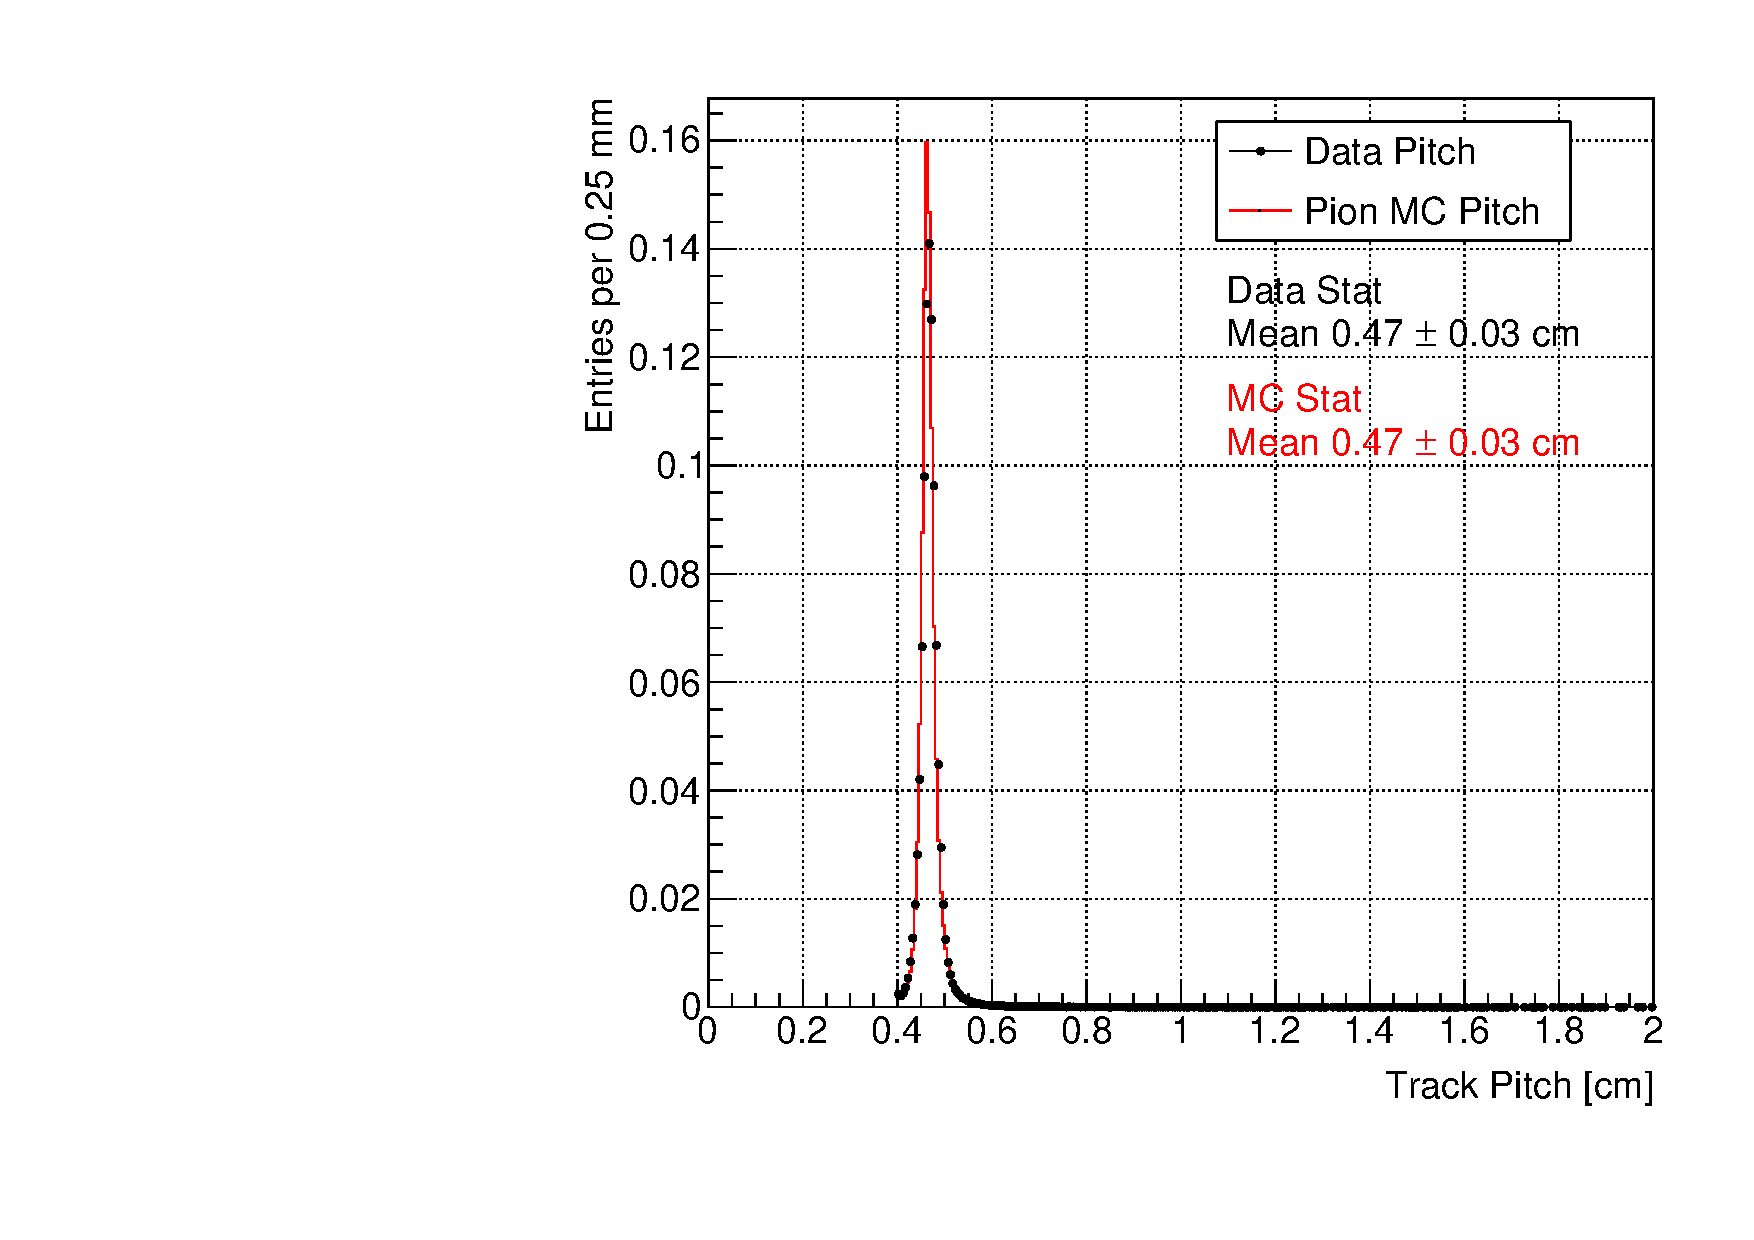
\includegraphics[width =0.4\textwidth ]{PitchPi}
\caption{\label{fig:pitch}  Pitch distribution for the Run II negative polarity data displayed in black, MC in red.}
\end{figure}
\begin{figure}
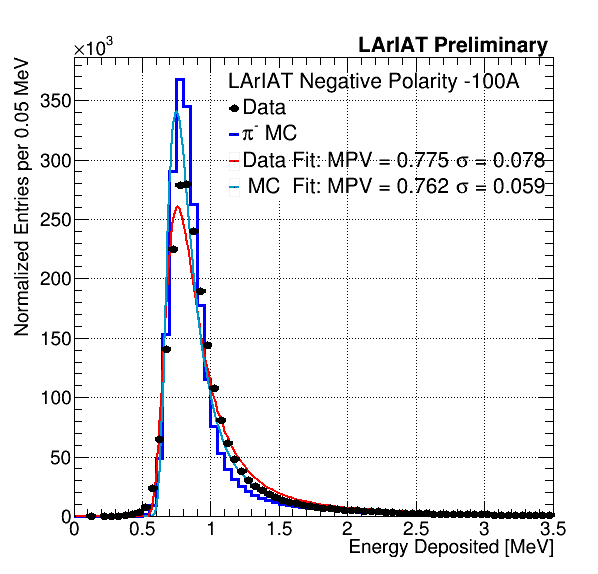
\includegraphics[width =0.4\textwidth ]{DepEnergy_Fit_v4100A.png}
\caption{\label{fig:enDep}  Energy deposition distribution in a single slice for Run II negative polarity data for the high energy tune displayed in black, MC in red. \textcolor{red}{(prettyfy)}}
\end{figure}

\begin{figure}
\centering
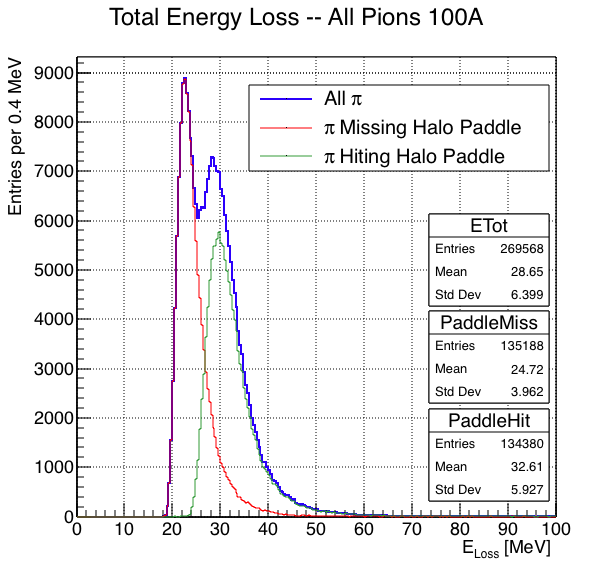
\includegraphics[width=0.45\textwidth]{E_loss100A.png}
\caption{\label{fig:ELoss100A}  True energy loss between the fourth wire chamber and the TPC front face according to the MC simulation of negative polarity data for the high energy tune. Two populations are visible, depending on the amount of un-instrumented material seen by the beamline pion. A scintillation paddle not used in this analysis (the halo paddle) sat between the DSTOF and the cryostat during Run II. The distribution for the pions missing the halo scintillation material is shown in red, and the distribution for the pions hitting the halo is shown in green, the distribution for the whole data sample is shown in blue. \textcolor{red}{(prettyfy)} }
\end{figure}



\subsection{\label{sec:Simulation}Simulation}
The LArIAT simulation toolkit used in this work is a combination of two Monte Carlo simulations: the G4Beamline Monte Carlo  [\textcolor{red}{cit needed}] and the Data Driven single particle Monte Carlo (DDMC).  G4Beamline simulates the beam collisions at the LArIAT target, the energy deposited by the particles in the beamline detectors, and the action of the magnets, effectively accounting for particle transportation through the beamline from the LArIAT target until the LArTPC. G4Beamline accounts for the beamline trigger and simulates the particle's composition in the beam. G4Beamline provides the relative percentages of particle species which the DDMC simulates downstream from the fourth wire chamber into the cryostat and into the LArTPC.  The measurement of the beamline particles' momentum and position at the fourth wire chamber performed on data serves as a basis for the DDMC event generation: the DDMC simulation samples from the joint distribution of the momentum and position measurements in data using a 5-dimensional hit-or-miss sampling procedure. This sampling generates MC events  with the same momentum and position distributions as data, with the additional benefit of accounting for the correlations among the considered variables. A LArSoft simulation module launches single particle MC from the location of the fourth wire chamber (100 cm upstream to the LArTPC) using the generated events. The particles are free to decay and interact in their path to the LArTPC according to the Geant4 simulation. We use the DDMC samples in several occasions: to propagate the estimated beamline background to the pion cross section, to calibrate the energy loss upstream of the LArTPC,  and to study the tracking and the calorimetric performance  in the LArTPC. 


\subsection{\label{sec:EventSelection}Beamline Event Selection}
\begin{table}
\caption{\label{tab:MCafterCutContaminants}Expected beamline composition for the selected events in the two energy tunes. \textcolor{red}{(update numbers)}}
\begin{ruledtabular}
\begin{tabular}{ l | l | l | l | l | l | l  |}
 &  \multicolumn{3}{c|}{Low Energy Tune} & \multicolumn{3}{c|}{High Energy Tune }\\
& MC $\pi$   & MC  $ \mu$ & MC  $e$ & MC  $\pi$ & MC  $\mu$ & MC  $e$  \\
\hline
&  &  &  & & &\\  
Expected &  &  &  & & &\\  
Composition&  88.5\%   & 8.2\%   & 3.3 \%   & 94.0\%	& 5.3\% & 0.7\%\\
in XS sample               &                      &                       &                   &                       &                        &\\  
&                      &                       &                   &                       &                        &\\  
\end{tabular}
\end{ruledtabular}
\end{table}

In data, the selection of beamline events proceeds as follows; we first reconstruct the beamline event, checking that the particle trajectory is plausible, which means rejecting events whose trajectory would seemingly  cross impenetrable material in the beamline, such as the magnets' steel. We minimize the occurrence of a pion capturing or decaying inside the chamber by a selection on the measured  beamline momentum; since pion capture and decay occur mainly at rest,  we select pions with momentum greater than 420 MeV/c, that is pions which are unlikely to stop inside the LArTPC.
For each of the negative polarity Run II events classified as $\pi/\mu/e$, we check the number of TPC tracks in the front portion of the TPC: in case more than four tracks are present in the first 14 cm we reject the event,  since the pile up of beam particles would affect the precision of the track reconstruction. The events that are matched to a TPC track and that survive the shower filter form the pool of beamline events for the cross section analysis. This pool is made of 40841 beamline pion candidates in data. 

In simulation, G4Beamline estimates the beam composition at the fourth wire chamber used to weight the number of electrons, muons and pions simulated with the DDMC. The simulated beamline events undergo the same selection flow as data: Table \ref{tab:MCafterCutContaminants} shows the predicted percentage of pions, muons and electrons in the pion beamline candidates selection. We feed beamline candidates to the ``thin slice method" machinery discussed in the next section in order to measure the negative pion total hadronic cross section. 



\begin{table}
\caption{\label{tab:beamlineDataSelection}Selection flow on the number of data events for Run-II Negative polarity towards the definition of beamline events for the pion cross section measurement.}
\begin{ruledtabular}
\begin{tabular}{l|r}
                                                        &  N Beamline Events     \\ \hline
Events Reconstructed in Beamline        &  158396     \\ \hline
Plausible Trajectory \& $p_{\text{Beam}}$ selection       &   147468    \\ \hline
Beamline $\pi^-/\mu^-/e^-$  Candidate  &   138481    \\ \hline
Events Surviving Pile Up Filter              &   108929    \\ \hline
Events with TPC Match                         &    41757     \\ \hline
Events Surviving Shower Filter             &    40841     \\ 
\end{tabular}
\end{ruledtabular}
\end{table}



\section{\label{sec:ThinSliceMethod}Thin Slice Method}
The pion interaction probability $P_{\text{Int}}$ in an argon target of thickness $\delta X$  is related to the cross section $\sigma_{\text{TOT}}$ by the following equation, 
\begin{equation}
P_{\text{Int}} = 1- e^{-\sigma_{\text{TOT}}\text{ } n \text{ }\delta X}
\label{eq:thinTargetXS}
\end{equation}
where $n$ is the density of the target centers. The density of target centers relates to the argon density $\rho$, the Avogadro number  $ N_{A} $ and the argon molar mass $m_A$ as $n=\frac{\rho N_{A} }{m_A}$.  The interaction probability $P_{\text{Int}}$ of pions on target can be statistically estimated as the ratio between the number of pions interacting in the thin target $N_{\text{Int}}$ (interacting flux) and the number of incident pions $N_{\text{Inc}}$ (incident flux). 
If the interaction length is significantly longer than the width of the target, i.e $\lambda_{\text{Int}} \gg \delta X$, we can assume that the target centers are uniformly distributed in the material and that no center of interaction sits in front of another -- the thin target approximation. In this case, it is possible to find a simple proportionality relationship between the cross section and the interaction probability by a Taylor expansion of the exponential function:
 \begin{equation}
 \sigma_{\text{TOT}}  = \frac{1}{n \text{ }\delta X}\frac{N_{\text{Int}}}{N_{\text{Inc}}}.
\label{eq:thinTargetXSSolved}
\end{equation}


Since the interaction length of pions in liquid argon is  expected  to be of the order of $\lambda_{\text{Int}} \sim 50$ cm, the LArIAT TPC and its 90 cm of depth do not represent a thin target. However, the granularity of the LArIAT LArTPC allows to assess the presence of a pion and measure its kinetic energy approximately every 4.7~mm along its trajectory in the detector's active volume. We can thus treat the argon volume as a sequence of many adjacent thin targets, recovering the thin target approximation in each argon slice. 


Each slice of argon {\emph{j}} represents an independent thin target experiment for which the incoming pion has a kinetic energy of  $E^{kin}_j$, measured according to Equation \ref{eq:KEj}. It should be noticed that each beamline pion candidate is likely to traverse multiple slices, thus participating in multiple independent thin target experiments at different kinetic energies. 
We apply the cross section calculation from Equation~\ref{eq:thinTargetXSSolved} in bins of kinetic energy: if a pion of kinetic energy $E^{kin}_j$ enters a slice, it contributes to the incident flux at the energy bin corresponding to $E^{kin}_j$.  Within the slice, the pion may or may not interact. If it does, it also contributes to the interacting flux at the same energy bin. If the pion does not interact,  it will enter the next slice and the evaluation of the fluxes is repeated for the new kinetic energy $E^{kin}_{j+1}$.   The kinetic energy   $E^{kin}_j$ is always greater than $E^{kin}_{j+1}$: while traveling in the TPC, the pion decreases its kinetic energy by ionizing and exciting the  argon. Thus, the same beamline pion will contribute to subsequent independent thin target experiments at progressively decreasing energies the further it travels downstream. 
We sum the contributions to the incident and interacting fluxes of all the beamline pion candidates in the selected sample to obtain $N_{\text{Int}}$ and  $N_{\text{Inc}}$ in bins of kinetic energy.\\
Since our goal is to measure the total interaction cross section independently  from the topology of the interaction, we determine that a pion interacted simply by requiring that the last point TPC track lies within the fiducial volume (FV), i.e. the volume contained within 1 cm from the TPC walls in the drift and vertical directions, 1 cm from the TPC front face and 4 cm from the TPC back face.
If the TPC track crosses the boundaries of the FV, the track is considered ``through going", no interaction point is found and no point external to the FV is consider for the evaluation of the fluxes. 


%\textcolor{red}{inefficiency and background}

%The only slices traversed by the pion beamline candidate track considered to fill the  $N_{\text{Int}}$ and  $N_{\text{Inc}}$ distributions are the ones contained in the fiducial volume. 
 
% A notable background pertinent only to the $N_{\text{Int}}$  distribution are cases in which the hadrons decays inside the TPC. In those cases in fact, the tracking ends inside the TPC but the interaction is not hadronic. The handling of decay background is treated in a slightly different way for the pion and kaon section, details can be found in sections \ref{ch:PionXSBkgSub} and \ref{ch:KaonXSRaw} respectively.


%\subsection{\label{sec:RawXS}Raw Cross Section}
\subsection{\label{sec:Corrections}Flux Corrections}
In the evaluation of the interacting and incident fluxes as a function of the pion kinetic energy,  two caveats are in place: a) residual muons and electrons are present in the beamline pion sample, b) TPC event reconstruction affects the evaluation of  $N_{\text{Int}}$ and $N_{\text{Inc}}$.
We then need to repackage Equation~\ref{eq:thinTargetXSSolved} at kinetic energy $E^{kin}_i$, as a function of the measured fluxes in data $N^{\text{Data}}_{\text{Int}}$ and $N^{\text{Data}}_{\text{Inc}}$, the corresponding corrections for beamline background contaminations $C^{\pi \text{MC}}_{\text{Int}}$ and $C^{\pi \text{MC}}_{\text{Int}}$ and corrections for reconstruction effects $\epsilon^{\text{Int}}$ and $\epsilon^{\text{Inc}}$ as follows

\begin{equation}
      \sigma^{\pi^-}_{TOT}(E^{kin}_{i})  = \frac{1}{n\text{ } \delta X}\frac{ \epsilon^{\text{Inc}}_i  \hspace{0.2cm} C^{\pi \text{MC}}_{\text{Int,i}}  \hspace{0.2cm} N^{\text{Data}}_{\text{Int,i}}  }{   \epsilon^{\text{Int}}_i \hspace{0.2cm} C^{\pi \text{MC}}_{\text{Inc,i}}  \hspace{0.2cm}  N^{\text{Data}}_{\text{Inc,i}} }.
\label{eq:C}
\end{equation}

where the subscript $i$ highlights that the quantities are evaluated separately in each kinetic energy bin.\\

\textbf{Corrections for Reconstruction Effects.}
We rely on the capacity of the tracking algorithm to identify the incoming pion in the TPC and to stop the tracking at the interaction point, evaluating whether or not the pion interacted.  The tracking algorithm has an intrinsic limitation in resolving shallow scattering angles, effectively determining a selection on the distribution of the scattering angle of hadronic interaction entering the cross section measurement.  We assess interaction angles smaller than 5$^\circ$ to be indistinguishable for the reconstruction; thus, we limit our ability to measure the cross section for interaction angles greater than 5.0 deg. 

The interacting and incident fluxes both depend on the efficiency of the tracking of finding the pion in the TPC and of finding the interaction point, albeit in a different way. If the tracking does not stop at an interaction point but keeps adding subsequent points to the pion trajectory, the missed interaction constitutes an inefficiency for the interaction flux and the slices corresponding to the extra trajectory points result in overcounts for the incident flux. On the contrary, if the tracking stops before an interaction point,  that flagged interaction point constitutes an overcount for the interaction flux and the missed subsequent slices represent an inefficiency for the incident flux. We encode both the inefficiency and overcount due to the reconstruction of the pion track in the flux corrections $\epsilon^{\text{Int}}_i$ and $\epsilon^{\text{Inc}}_i$. We use a sample of DDMC pions to evaluate the flux corrections as follows,

\begin{equation}
 \epsilon^{\text{Int}}_i  =  \frac{N^{\text{ Reco MC $\pi$}}_{\text{Int,i}}}{ N^{\text{ True MC  $\pi$}}_{\text{Int,i}}  } \hspace{0.5cm}\text{and}\hspace{0.5cm}  \epsilon^{\text{Inc}}_i  =  \frac{N^{\text{ Reco MC $\pi$}}_{\text{Inc,i}}}{ N^{\text{ True MC  $\pi$}}_{\text{Inc,i}}  },
\end{equation}

where $N^{\text{ True MC  $\pi$}}_{\text{Int,i}}$ is the expected number of interacting pions at the kinetic energy $E^{kin}_i$ according to the Geant4 10.03.p1 FTFP\_BERT interaction model and  $N^{\text{ Reco MC $\pi$}}_{\text{Int,i}}$ is the number of reconstructed interacting pions at the same kinetic energy; analogous definitions apply to the correction on the incident flux. \\




\textbf{Corrections for Beamline Background.}
Even if pions are by far the biggest beam component in the selected beamline candidates, residual muons and electrons are present in the sample. We estimate %the muon and electron contributions to the incident and interacting flux in data through MC. Our goal is to estimate  
the pion content $C^{\pi \text{MC}}_{\text{Int,i}}$ and  $C^{\pi \text{MC}}_{\text{Inc,i}}$, i.e. the percentage of pion entries in the interacting and incident flux at each kinetic energy bin $E^{kin}_i$ on Monte Carlo; we then apply these corrections to the corresponding kinetic energy bin in data.  

We simulate pions, muons and electrons with the DDMC, using the relative abundance predicted by the beamline simulation.  We feed pions, muons and electrons to the thin slice method machinery, estimating the interacting and incident fluxes for each particle species.

We calculate the relative pion content for the interacting and incident flux  as
\begin{equation}
C^{\pi \text{MC}}_{\text{Int,i}}  =  \frac{N^{\pi \text{MC}}_{\text{Int,i}}}{ N^{\text{TOT MC}}_{\text{Int,i}} } 
\end{equation}
and 
\begin{equation}
C^{\pi \text{MC}}_{\text{Inc,i}}  =  \frac{N^{\pi \text{MC}}_{\text{Inc,i}}}{ N^{\text{TOT MC}}_{\text{Inc,i}} } 
\end{equation}

where 
$N^{\text{TOT MC}}_{\text{Int,i}}$ and $N^{\text{TOT MC}}_{\text{Inc,i}}$ are the the sum of the MC pion, muon and electron contributions to the interacting and incident flux respectively, while $N^{\pi}_{\text{Int,i}}$ and $N^{\pi}_{\text{Inc,i}}$ represent the sole MC pion contribution. Once we evaluate the $C^{\pi \text{MC}}_{\text{Int,i}}$ and  $C^{\pi \text{MC}}_{\text{Inc,i}}$ separately, we use their ratio to correct the measured raw cross section. Muons represent the biggest contribution to beamline backgrounds. The muon presence in the sample tends to lower the measured raw cross section; this is because most of the muons will cross the TPC without stopping, contributing almost exclusively to the incident flux. 



\subsection{\label{sec:Corrections}Treatment of the uncertainties}
We calculate the statistical uncertainty for a given kinetic energy bin of the cross section propagating the statistical uncertainty on $N_{\text{Int,i}}$ and $N_{\text{Inc,i}}$.  Since the number of incident particles in each energy bin is given by a simple counting, we assume that $N_{\text{Inc,i}}$ is distributed as a poissonian with mean and variance equal to $N_{\text{Inc,i}}$ in each bin.  
On the other hand, $N_{\text{Int,i}}$ follows a binomial distribution: a particle in a given energy bin might or might not interact.  The variance for the binomial is given by  
\begin{equation}
\text{\textsf{Var[}} N_{\text{Int,i}} \text{\textsf{]}}
 = N_{\text{Inc,i}}P_{\text{Int,i}}(1-P_{\text{Int,i}}),
\label{eq:binVar}
\end{equation}

where  $P_{\text{Int,i}}$ is estimated by $\frac{ N_{\text{Int,i}}}{N_{\text{Inc,i}}}$ and the number of tries corresponds to $N_{\text{Inc,i}}$. $N_{\text{Inc,i}}$ and $N_{\text{Int,i}}$ are not independent. In fact, populating a given bin for the interacting flux always implies at least populating the same bin in the incident flux  (and possibly other incidents bins at higher energies). Thus, we conservatively calculate the statistical uncertainty on the cross section as 
\begin{equation}
\frac{\delta\sigma^{Stat}_{TOT}(E^{kin}_i)}{\sigma^{Stat}_{TOT}(E^{kin}_i)} =  \frac{\delta N_{\text{Int,i}}}{N_{\text{Int,i}}}+\frac{\delta N_{\text{Inc,i}}}{N_{\text{Inc,i}}}
\end{equation}
where:
\begin{eqnarray}
\delta N_{\text{Inc,i}} = \sqrt[]{N_{\text{Inc,i}}} \\
\delta N_{\text{Int,i}} = \sqrt[]{N_{\text{Int,i}}\Big(1-\frac{ N_{\text{Int,i}}}{N_{\text{Inc,i}}}\Big)}.
\end{eqnarray} \\


The evaluation of the systematic uncertainty results from the propagation to the cross section of the uncertainty associated with  the track pitch  ($\delta X = 0.47 \pm 0.03 $ cm, shown in Figure \ref{fig:pitch}),  the measured kinetic energy at each argon slab,  the  beam composition and the correction for reconstruction effects. 

The uncertainty on the kinetic energy of a pion candidate at the j$^{th}$ slab of argon  is given by

\begin{eqnarray}
\delta E^{kin}_{j} &=& \sqrt{\delta p_{\text{Beam}}^2 + \delta E_{\text{Loss}}^2 +  \delta \Big(\sum_{n < j} E_{\text{Dep},n}\Big)^2}, 
%&=& \sqrt{(2\% \text{ }p_{Beam})^2 +  ( 6 \text{ [MeV]})^2 +  (j-1)^2 (\sim0.08\text{ [MeV]})^2}.
\end{eqnarray}

where $\delta p_{\text{Beam}} = 2\%$ $p_{\text{Beam}}$, $\delta E_{\text{Loss}}$ is the width of the distribution in Figure \ref{fig:ELoss100A}, $\delta \Big(\sum_{n < j} E_{\text{Dep},n}\Big)$  is the uncertainty associated to energy deposited by the pion from the TPC front face to the $j^{th}$ slice; we calculate this last uncertainty as  the sum of $\delta E_{\text{Dep},n}$, that is the width  of the  distribution of energy deposited in a single slice, see Figure \ref{fig:enDep}. We propagate the uncertainty on the kinetic energy to the cross section by varying the energy measurement $E^{kin}_{j}$ at each argon slab and evaluating the cross section in three cases: first we assign the measured $E^{kin}_{j}$, then  $E^{kin}_{j} + \delta E^{kin}_{j}$, and finally  $E^{kin}_{j} - \delta E^{kin}_{j}$. The difference between the cross section values using the $E^{kin}_{j}$ sampling and the maximum and minimum values in each bin determines the systematic uncertainty. We asses the systematic uncertainty on the beam composition in a similar fashion; we vary beamline muon and electron content by 20\% and evaluate the subsequent cross section variation.  The systematics on the correction for reconstruction effects is estimated by varying Geant4 cascade model from our default (FTFP\_BERT) to QGSP\_BERT.  \textcolor{red}{we should come up with something better}. 



\section{\label{sec:Results}Result}
% sections are not used for PRL papers
The top plot of Figure \ref{fig:epsart} shows the measurement of the ($\pi^-$-Ar) total hadronic cross section,  for  scattering angles greater than 5$^\circ$, as the result of the fluxes' corrections and combination of the low and high energy tune data sets. The statistical uncertainty and the sum in quadrature of statistical and systematic uncertainty are shown in black; for reference, the green line represents the Geant4 prediction based on the FTFP\_BERT cascade model  for angle scattering greater than 5$^\circ$. 
With the exception of the highest energy bins (energy greater than 800 MeV), the systematic uncertainties are the dominant uncertainties; the lion's share of the systematic uncertainty results from our uncertainty on the beam composition \textcolor{red}{[cross check needed]}. The bottom panel of Figure  \ref{fig:epsart} shows the relative deviation between the measured cross section and  Geant4 predicted cross section.
Our measurement is in agreement with the Geant4 predictions derived from historic measurements on lighter and heavier nuclei in the 350-1050 MeV region, while a shape difference arises at lower energies where the cross section is boosted by the presence of the delta resonance.

Table \ref{tab:XSsummary} summarizes the cross section as a function of kinetic energy and  the associated total uncertainty; it also reports the recorded fluxes,  beamline background corrections and the  corrections due to the reconstruction of the pion track.\\


\begin{figure}
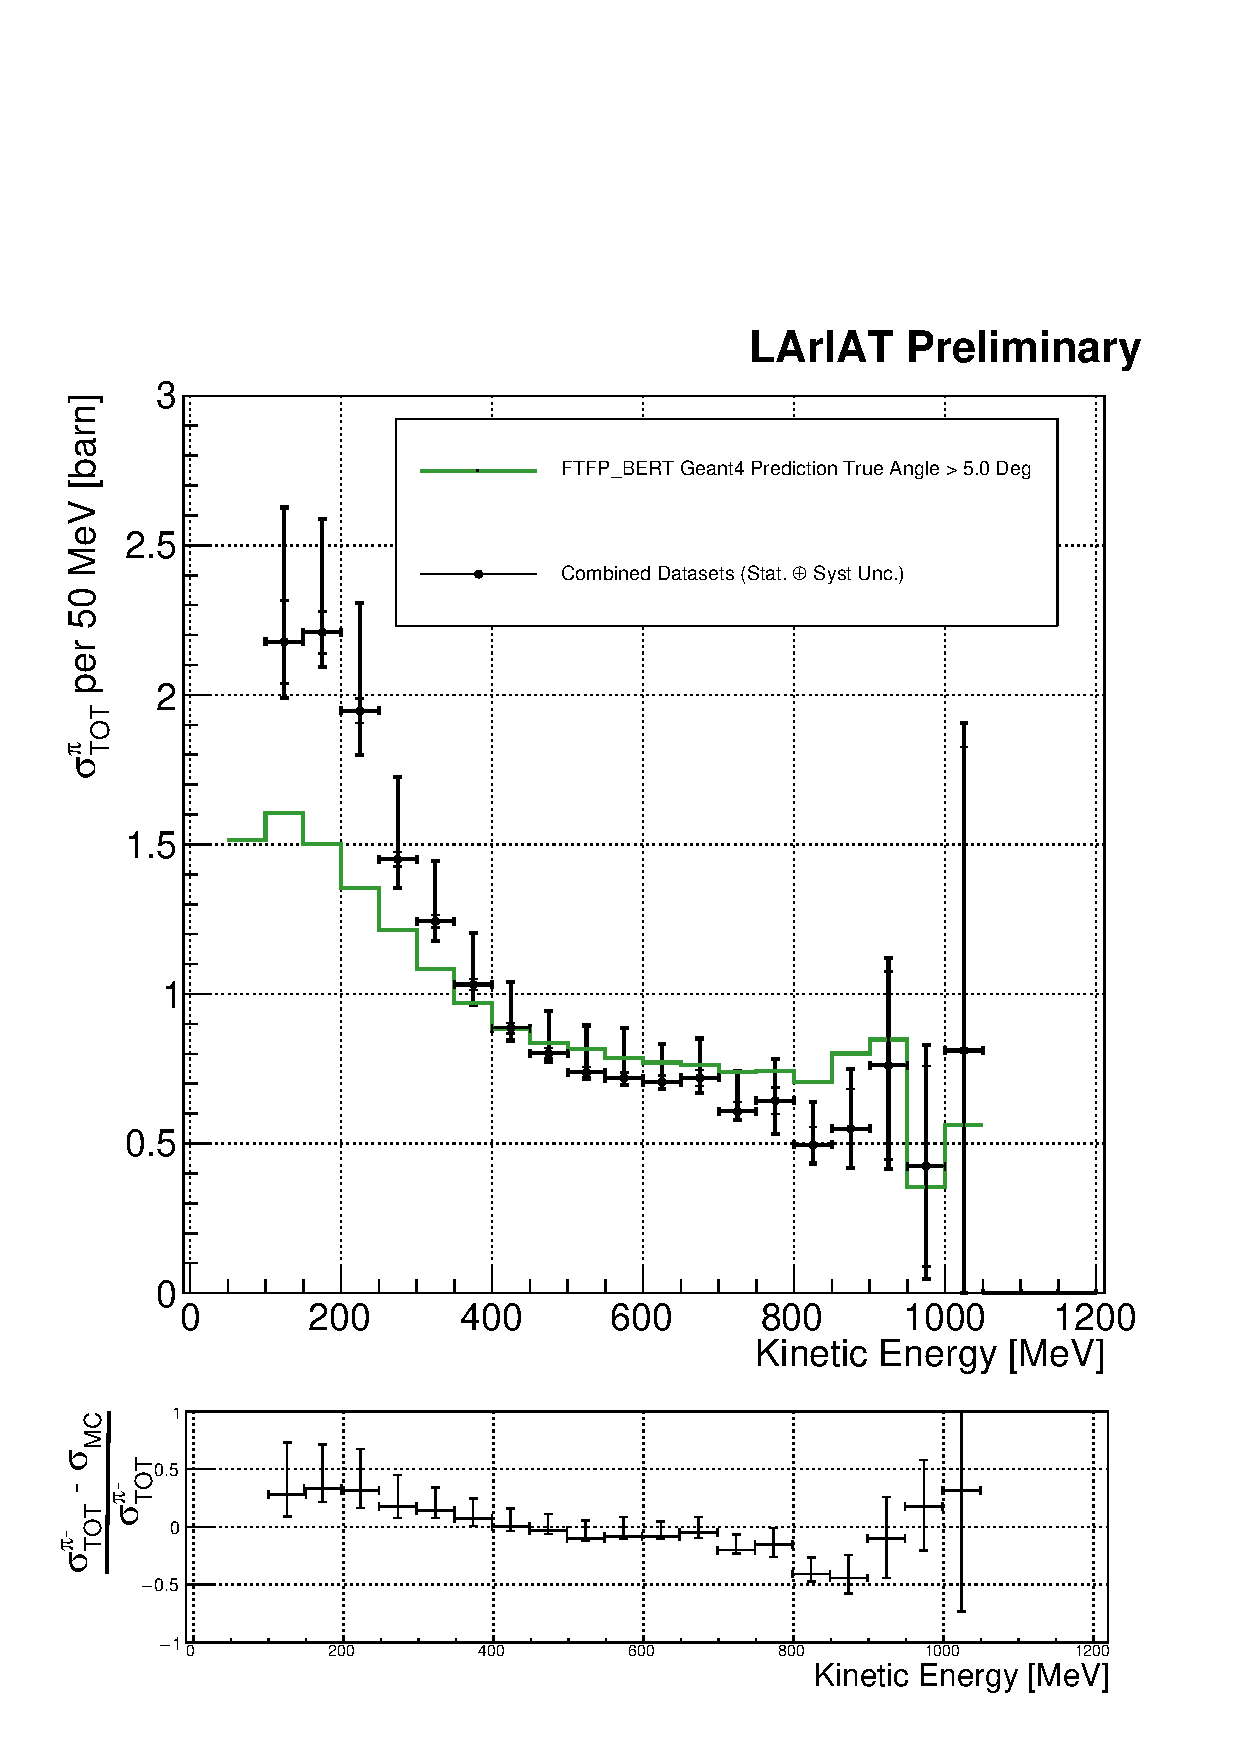
\includegraphics[width =0.4\textwidth ]{TheRealMoneyPlot}
\caption{\label{fig:epsart} Top: ($\pi^-$-Ar) total hadronic cross section for  scattering angles greater than 5$^\circ$ measured in the combined sample, statistical uncertainty and systematic uncertainty in black. The Geant4 prediction for the total hadronic cross section for angle scattering greater than 5$^\circ$ is displayed in green. Bottom: relative difference between the measured cross section and the Geant4 prediction. }
\end{figure}

\begin{table*}
\caption{\label{tab:XSsummary} Results summary. }
\begin{ruledtabular}
\begin{tabular}{ccccccccc}
$[E^{kin}_{\text{MIN}}, E^{kin}_{\text{MAX}}]$ & $\sigma_{\text{TOT}}$ & Stat $\bigoplus$ Syst  & $N^{ \text{Data}}_{ \text{Int}}$
& $N^{ \text{Data}}_{ \text{Inc}}$ & $C^{\pi \text{MC}}_{\text{Int}}$  & $C^{\pi \text{MC}}_{\text{Inc}}$ & $ \epsilon^{\text{Int}} $ & $\epsilon^{\text{Inc}}$ \\ 
(MeV)& (Barn)& Uncertainty (Barn) & & & & & \\\hline
& & & & & & &\\
 $[100,150]$ &1&+20/-10 & & & & & &\\
\end{tabular}
\end{ruledtabular}
\end{table*}

\clearpage
\input acknowledgement.tex   % input acknowledgement
\bibliography{bib.bib}

%\begin{thebibliography}{99}

%  \bibitem{LArIATDet}
%    Standard LArIAT detector reference:  \\
%R. Acciarri {\sl et al.} (LArIAT Collaboration),
%hopefully we'll have one soon.

%  \bibitem{LArSoft}
%    Standard LArSoft reference:  \\
%hopefully we'll have one soon.

% \end{thebibliography}

\end{document}
%
% ****** End of file template.aps ******
